%! TEX root = **/010-main.tex
% vim: spell spelllang=en:

\subsection{K-NN}%
\label{sub:knn}
To make our KNN performance a little better we tried different dimensionality reduction techniques and compared their results.
The three candidates were PCA, that's the most common and the one we've seen in class, LDA, that's closely related to PCA but actively tries to find differences between the classes and finally NCA, which is a more complex method that could actually substitute KNN and uses a pretty related algorithm called stochastic nearest neighbours.

We tried values of K ranging from 1 to 50 with both weighted and unweighted KNN for the three dimensionality reduction methods and got this output:
\begin{figure}[H]
    \centering
    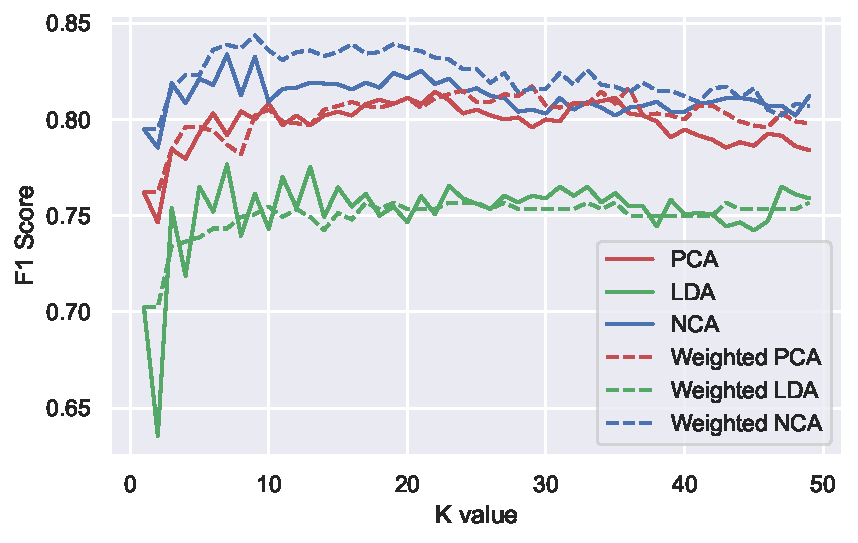
\includegraphics{knn}
    \caption{weighted and unweighted knn with PCA, LDA and NCA}%
    \label{fig:knn_pca_lda_nca}
\end{figure}

\fresults{ 367 &  41 \\ 22 & 170 }{0.895}{0.844}

As we see, NCA gets the best result, and the weighted variant of it goes a little bit further giving us even better results, as for the K value, we see that the f1 score is bad for very low values of K, gets maximized at K\approx9 and then it stays stable for the tested range.
% Description of procedure followed for choosing the best k-parameter. Show  a  graph  with  varying  k.  
% Have  you  adjusted  other  parameters  as distance measure? 
% Have you considered removal of irrelevant features if accuracy  is  poor  compared  with  other  approaches?   
% (remember  that  k-nn  is  sensible  to  irrelevant  features  when  computing  distance  to  closest examples

% cf - acc - f1
%\fresults{ 384 &  24 \\ 21 & 171 }{0.925}{0.883}